\documentclass[a4paper, 10pt]{article}
\usepackage[utf8]{inputenc}
\usepackage{graphicx}
\usepackage{hyperref}
\usepackage{amsmath}
\usepackage{amssymb}
\usepackage{geometry}
\usepackage{flafter}
\usepackage{float}

% Imposta i margini
\geometry{
  a4paper,
  left=25mm,
  right=25mm,
  top=30mm,
  bottom=30mm
}

\begin{document}

\begin{titlepage}
    \centering
    \vspace*{1cm}
    
    \Huge
    \textbf{Kernelized Linear Classification}
    
    \vspace{0.5cm}
    \LARGE
    Implementing classification algorithms from scratch
    
    \vspace{1.5cm}
    
    \textbf{Loris Palmarin - 32349A}
    
    \vfill
    
    \Large
    \textbf{Data Science for Economics\\}
    \textbf{Department of Economics, Management and Quantitative Methods\\}
    \textbf{Department of Computer Science "Giovanni degli Antoni"\\}
    \textbf{Università degli Studi di Milano}
    
    \vspace{0.8cm}
    
    \Large
    \textbf{Academic Year 2023/2024}
    
\end{titlepage}

\newpage

\thispagestyle{empty}

\vspace*{\fill}
\noindent
\textit{I declare that this material, which I now submit for assessment, is entirely my own work and has not been taken from the work of others, save and to the extent that such work has been cited and acknowledged within the text of my work. I understand that plagiarism, collusion, and copying are grave and serious offences in the university and accept the penalties that would be imposed should I engage in plagiarism, collusion or copying. This assignment, or any part of it, has not been previously submitted by me or any other person for assessment on this or any other course of study.}



\vspace{1.5cm}
\noindent
Link to the repository:\\
\url{https://github.com/lorispalmarin/machlear-dse2}

\vspace*{\fill}

\newpage

\tableofcontents

\newpage

\section*{Introduction}
\addcontentsline{toc}{section}{Introduction}
The primary objective of this project is to develop various algorithms for classification using the Python programming language. After implementing these algorithms, the goal is to calculate the misclassification rate and determine which model performs best.

The implementation requires avoiding libraries such as SciKit Learn, and instead, building all models from scratch. This approach allows for a deeper exploration of different implementations and aids in identifying the most effective solution for the problem at hand.

The key questions addressed in this project include:
\begin{itemize}
    \item How does the misclassification rate vary depending on the model used?
    \item How significant is the impact of effective hyperparameter tuning on the performance of each model?
\end{itemize}

In attempting to answer these questions, the work is structured as follows:

First, an exploratory data analysis (EDA) is conducted to perform the necessary preprocessing steps and avoid data leakage between the training and test sets.

The implementation of the algorithms is then divided into three main parts:

\begin{itemize}
    \item In the first part, the Perceptron, Support Vector Machines (SVMs) using the Pegasos algorithm, and regularized logistic classification are developed. After implementing these algorithms from scratch, their performances and the best parameters for each model are evaluated.
    \item In the second part, polynomial feature expansion of degree two is applied, and the aforementioned models are re-implemented to assess whether the polynomial expansion improves the predictive capabilities of the models. During this process, the linear weights corresponding to the various numerical features found after the training phase are utilized, stored, and analyzed for their significance.
    \item In the third and final part, kernel methods are implemented. Specifically, the kernelized Perceptron with Gaussian and polynomial kernels, and the kernelized Pegasos algorithm for SVMs, using both polynomial and Gaussian kernels, are developed. The performance of these models is analyzed, and the optimal parameters are identified.
\end{itemize}

Finally, a comprehensive analysis of the predictive capabilities of the various models is presented, aiming to identify the best-performing models in this context.


\newpage
\section{Preprocessing}

In this section, the dataset was carefully examined and preprocessed to ensure that the models could be trained on clean and meaningful data. The process involved handling missing values, analyzing distributions, detecting and handling outliers, and ensuring that the features were appropriately scaled.

\subsection{Initial Data Exploration}

The dataset initially contained 11 columns, including the target variable \texttt{y} and 10 numerical features labeled \texttt{x1} to \texttt{x10}. To get an initial sense of the data, the first few rows were printed, and a statistical summary was generated to understand the basic characteristics of the features (fig.\ref{fig:mesh1}).


\begin{figure}[H]
    \centering
    \includegraphics[width=0.6\textwidth]{images/statsumm.png}
    \caption{Statistical summary}
    \label{fig:mesh1}
\end{figure}

The statistical summary revealed that the features had varying scales, ranges, and distributions. For example, the mean and standard deviation for \texttt{x1} were notably different from those of \texttt{x10}, indicating that feature scaling would be necessary before feeding the data into any machine learning model.

\subsection{Handling Missing Values}

Any potential missing values were handled by dropping rows with NA values to ensure that the dataset was complete for subsequent analysis. Fortunately, the dataset did not contain any missing values after this operation.


\subsection{Analyzing Distributions and Outliers}

To better understand the distribution of each feature and identify potential outliers, histograms and boxplots were generated for all numerical features. This visualization step was crucial for identifying skewed distributions and features with significant outliers.

\begin{itemize}
    \item \textbf{Histograms} (fig.\ref{fig:histograms}): The histograms revealed that several features, such as \texttt{x2} and \texttt{x9}, had skewed distributions, which could affect the performance of certain models if not addressed.
    \item \textbf{Boxplots} (fig.\ref{fig:boxplots}): The boxplots further highlighted the presence of outliers in features like \texttt{x2}, \texttt{x7}, \texttt{x8}, and \texttt{x9}. These outliers were subsequently handled using the Interquartile Range (IQR) method.
\end{itemize}

\begin{figure}[H]
    \centering
    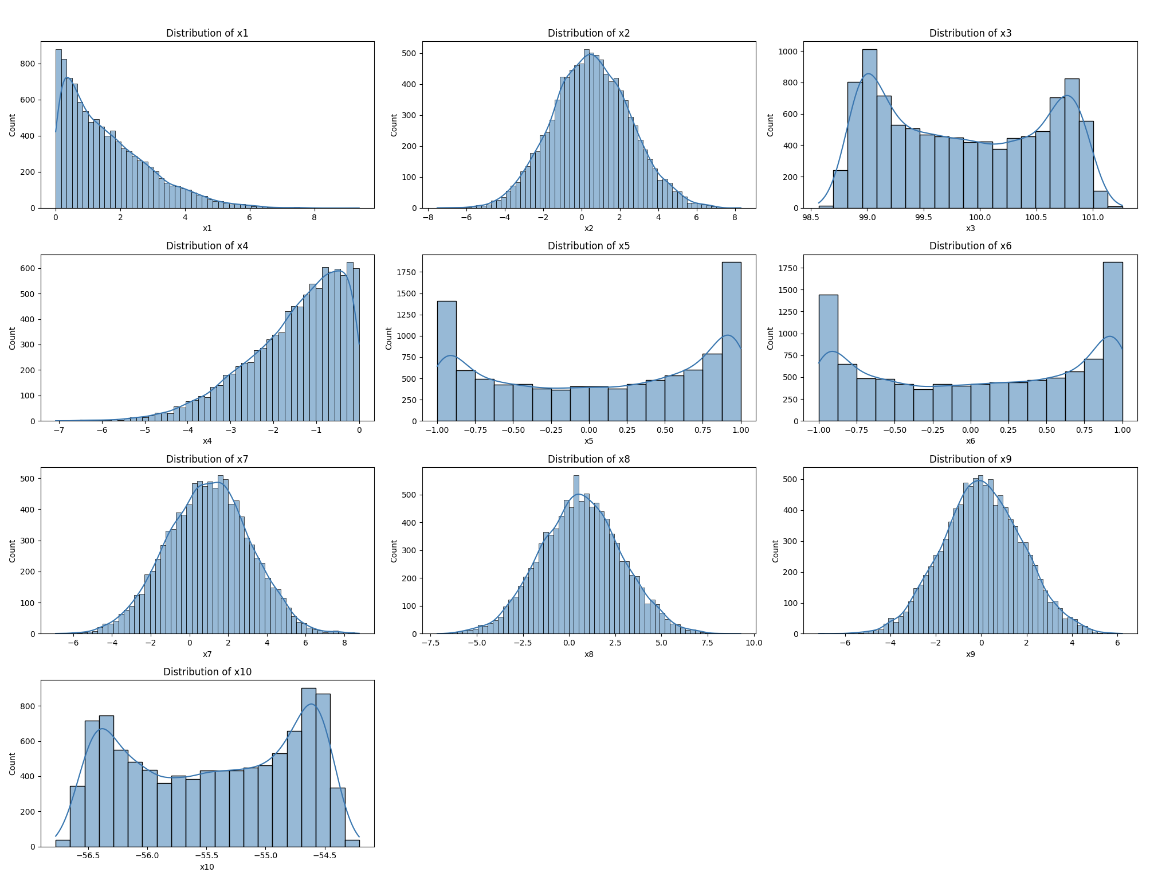
\includegraphics[width=0.6\textwidth]{images/histograms.png}
    \caption{Histograms}
    \label{fig:histograms}
\end{figure}
\begin{figure}[H]
    \centering
    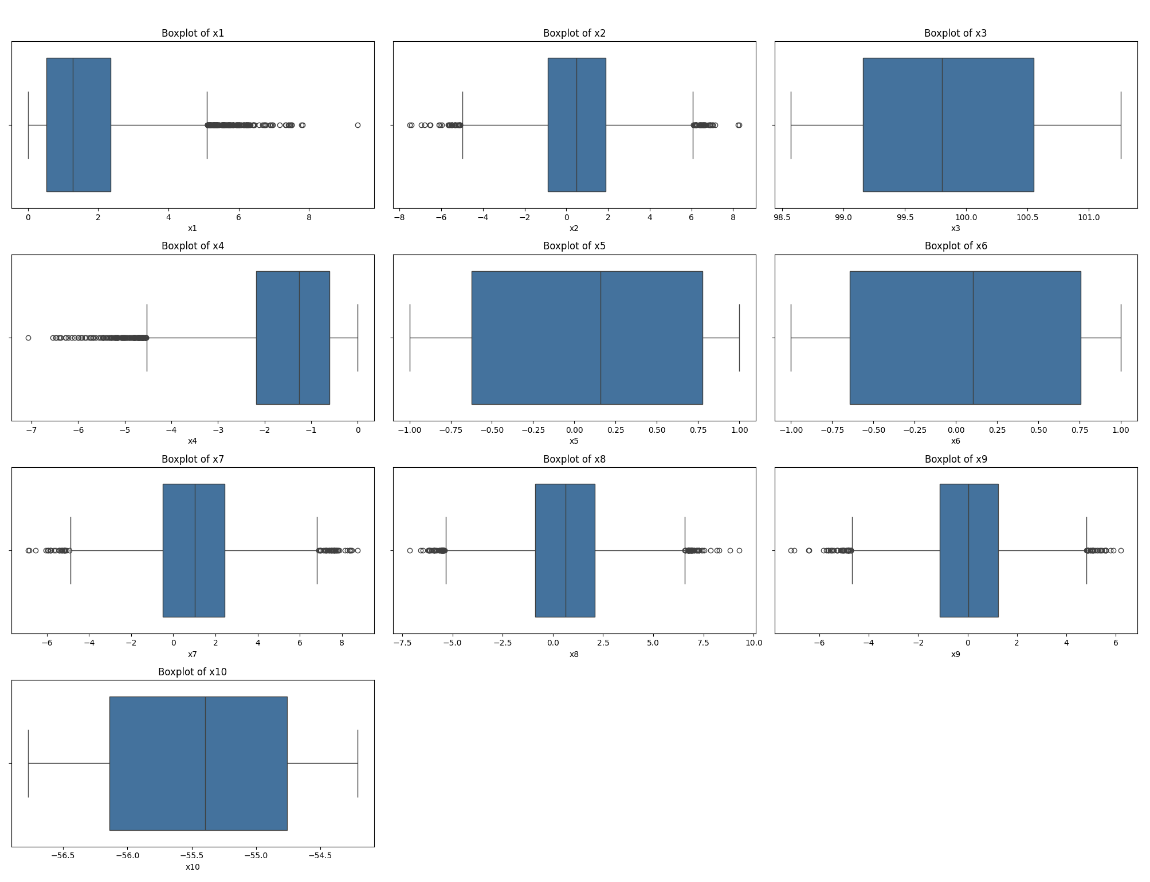
\includegraphics[width=0.6\textwidth]{images/boxplots.png}
    \caption{Boxplot}
    \label{fig:boxplots}
\end{figure}

After removing outliers, the dataset size was reduced slightly, ensuring that extreme values did not unduly influence the models.

\subsection{Correlation Analysis}

A correlation matrix was computed and visualized to detect highly correlated features. Highly correlated features can introduce multicollinearity, which can degrade the performance of certain machine learning models.

\begin{itemize}
    \item \textbf{Before Processing} (fig.\ref{fig:corrpre}): The initial correlation matrix showed a high correlation between \texttt{x3}, \texttt{x6} and \texttt{x10}.
    \begin{figure}[H]
    \centering
    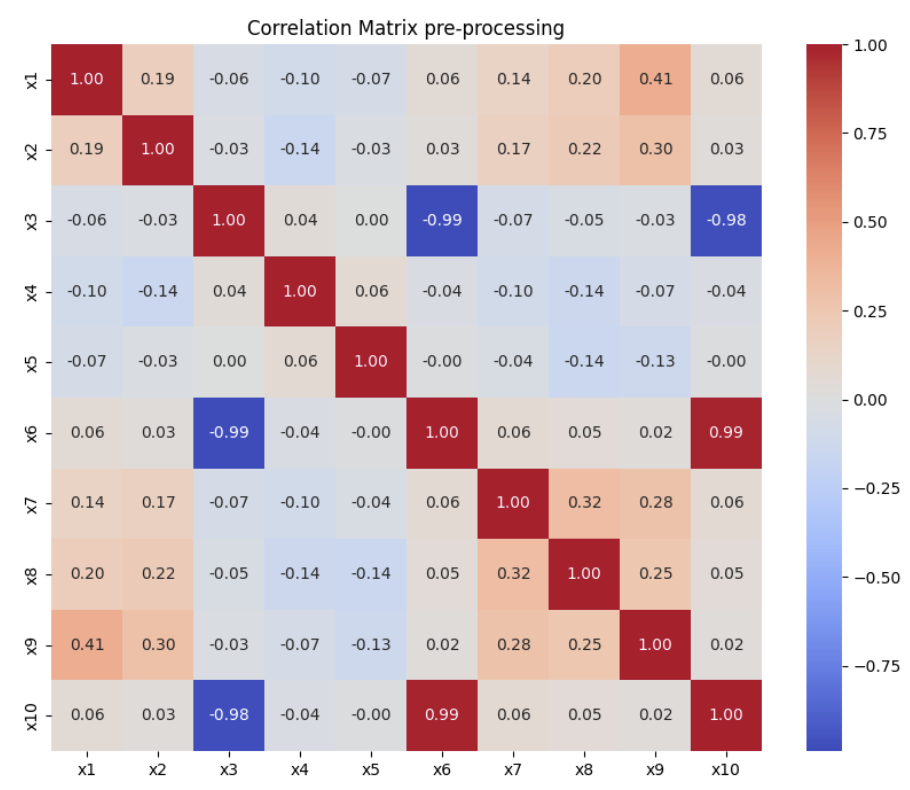
\includegraphics[width=0.6\textwidth]{images/corrpre.png}
    \caption{Correlation pre-processing}
    \label{fig:corrpre}
\end{figure}
    \item \textbf{After Processing} (fig.\ref{fig:corrpost}): To address this issue, the features \texttt{x6} and \texttt{x10} were removed. A new correlation matrix was generated to verify the absence of multicollinearity among the remaining features.
    \begin{figure}[H]
    \centering
    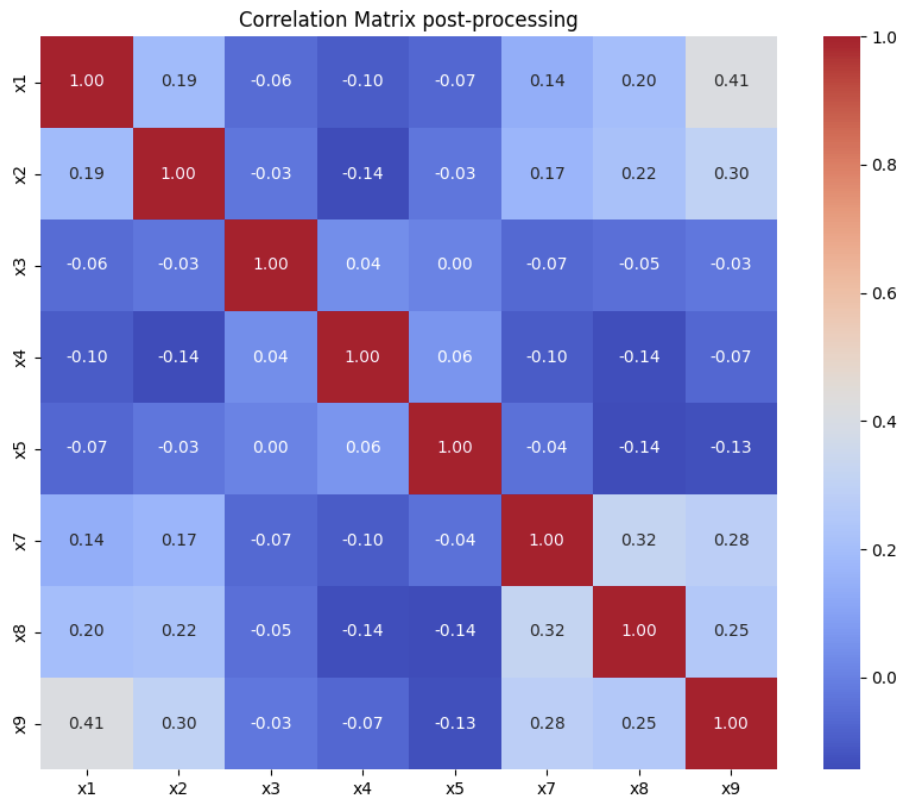
\includegraphics[width=0.6\textwidth]{images/corrpost.png}
    \caption{Correlation post-processing}
    \label{fig:corrpost}
\end{figure}
\end{itemize}


This step ensured that the remaining features were not overly correlated, which could otherwise lead to redundancy in the model training process.

\subsection{Data Splitting}

The cleaned dataset was then split into training and testing sets, with 80\% of the data used for training and 20\% reserved for testing. \textbf{This split was done to avoid any data leakage, ensuring that the test set remains entirely separate and unseen during the training process}.



\subsection{Feature Scaling}

Given the different scales of the features, feature scaling was performed using standardization. This step was crucial to ensure that all features contributed equally to the model's learning process.
The scaling was fitted on the training data, and the same transformation was applied to both the training and test sets to prevent data leakage.




\textbf{Feature scaling was performed in such a way that the scaler was fitted on the training set only and then applied to the test set, thereby avoiding data leakage}. After scaling, a final statistical summary was generated to confirm that all features had a mean of 0 and a standard deviation of 1, as expected from the standardization process.

\subsection{Model optimization and performance evaluation}
In this project, the algorithms are optimized using 5-fold cross-validation, with accuracy as the primary evaluation metric during the training and validation phases. In the context of \(k\)-fold cross-validation, the dataset is divided into \(k\) subsets, or "folds." The model is trained on \(k-1\) folds and validated on the remaining fold, with this process repeated \(k\) times to ensure robustness. The accuracy metric, defined as

\[
\text{Accuracy} = \frac{\text{Number of Correct Predictions}}{\text{Total Number of Predictions}},
\]

is used to assess the proportion of correctly predicted instances during this phase.

However, to evaluate the final performance of the models on the unseen test set, we employ the 0-1 loss, also known as the misclassification rate. This metric is defined as:

\[
\ell(y, \hat{y}) = 
\begin{cases} 
0 & \text{if } y = \hat{y}, \\
1 & \text{otherwise}.
\end{cases}
\]

where \(y_i\) represents the true label and \(\hat{y}_i\) is the predicted label. The 0-1 loss effectively measures the proportion of incorrect predictions, serving as a direct indicator of the model's misclassification rate on the test set.

When implementing grid search with cross-validation, it was essential to ensure that the different cross-validation folds and hyperparameter combinations were completely independent from each other. To achieve this, I introduced the model.reset() function inside the hyperparameter iteration loop. This function ensures that the internal state of the model is reset to the initial condition before each new parameter combination. In this way, the results obtained from one fold or parameter combination are prevented from influencing subsequent ones, preserving the integrity of the cross-validation results and ensuring a correct and unbiased evaluation of the model performance.

\newpage
\section{Implementing Algorithms for Linear Classification}

\subsection{Perceptron}

The Perceptron algorithm is one of the simplest linear classifiers and is a fundamental model for understanding more complex classification algorithms. It works by iteratively adjusting a weight vector to correctly classify training examples. The Perceptron decision boundary is a hyperplane that separates the data into two classes. \par

Mathematically, the Perceptron tries to find a weight vector \(\mathbf{w}\) such that for a set of training examples \(\{(\mathbf{x}_i, y_i)\}_{i=1}^m\), where \(\mathbf{x}_i \in \mathbb{R}^d\) and \(y_i \in \{-1, 1\}\), the following condition holds:

\[
y_i (\mathbf{w}^\top \mathbf{x}_i) > 0, \quad \forall i = 1, \dots, m
\]

If this condition is not satisfied for a particular example \({x}_i\), the algorithm updates the weight vector \({w}\) by adding \(y_i \mathbf{x}_i\). This process is repeated for a specified number of epochs or until the algorithm converges, i.e. no errors are made in an entire pass through the training data.

\subsubsection{Implementation of the Perceptron Algorithm}

The Perceptron algorithm implemented in this project was designed to run a maximum number of epochs, with the option to stop early if convergence is achieved before the maximum epoch limit. The cross-validation process was conducted with 5 folds to evaluate the performance of the model. The key parameters optimized during cross-validation were the number of epochs.
\par
The cross-validation results for different epoch values are as follows:

\begin{itemize}
    \item \textbf{1000 Epochs:}
    \begin{itemize}
        \item Accuracy for each fold: [0.6293, 0.5663, 0.6088, 0.5576, 0.5524]
        \item Average cross-validation accuracy: 0.5829
    \end{itemize}
    \item \textbf{2000 Epochs:}
    \begin{itemize}
        \item Accuracy for each fold: [0.6265, 0.5759, 0.6937, 0.5937, 0.6104]
        \item Average cross-validation accuracy: 0.6198
    \end{itemize}
    \item \textbf{5000 Epochs:}
    \begin{itemize}
        \item Accuracy for each fold: [0.6145, 0.5283, 0.6789, 0.6220, 0.5441]
        \item Average cross-validation accuracy: 0.5976
    \end{itemize}
\end{itemize}

It's important to underline that none of the different parameters reached convergence. This fact, combined to the low accuracy, suggests that data aren't linearly separable and that the model isn't complex enough to find a good classifier.

\begin{figure}[H]
    \centering
    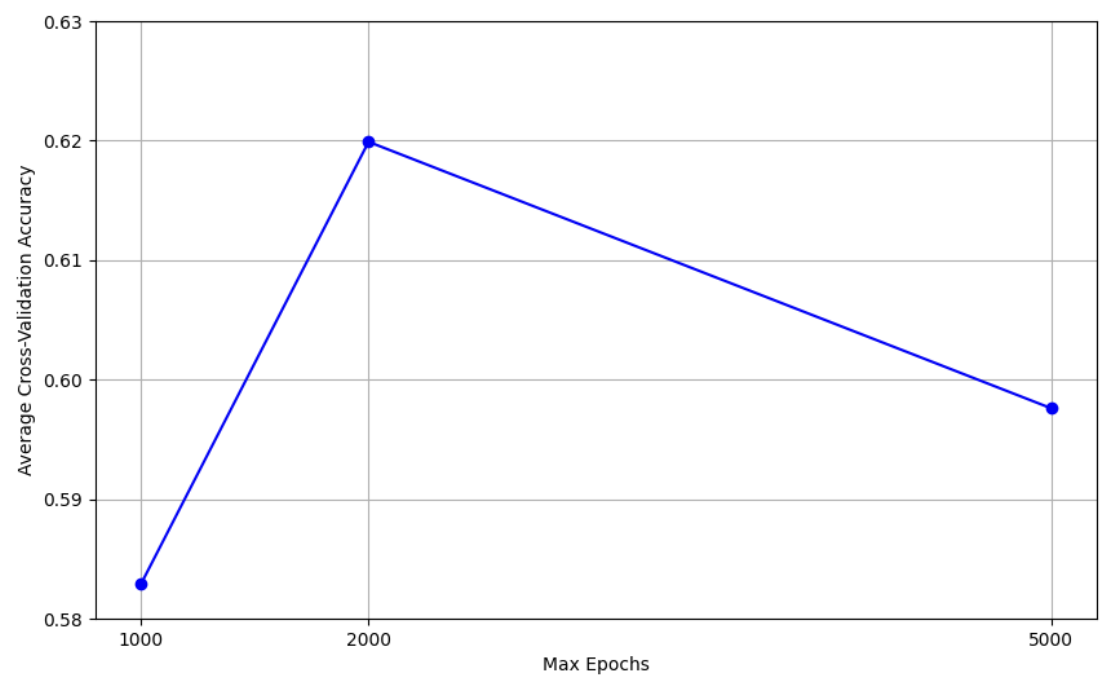
\includegraphics[width=0.6\textwidth]{images/perceptron.png}
    \caption{Accuracy vs Max Epochs}
    \label{fig:accuracyperc}
\end{figure}

\subsubsection{Hyperparameter Tuning and Overfitting/Underfitting Analysis}

In the hyperparameter tuning process, the number of epochs was selected as the key parameter to optimize. This is a crucial aspect since too few epochs could lead to an under-trained model (underfitting), while too many could lead to an over-trained model (overfitting).

In this case, the results indicate that 2000 epochs represent a good compromise between accuracy and computational complexity. The model with 2000 epochs ended faster and achieved an average accuracy better than the others, as seen in Fig.\ref{fig:accuracyperc}. This suggests that beyond a certain number of epochs, the Perceptron does not improve its performance, and further training only leads to an increase in computation time without a real benefit in terms of accuracy.

Furthermore, it is important to consider the difference between the performance in cross-validation and on the test set. After choosing the 2000-epoch model based on the cross-validation results, the final training and evaluation was performed on the test set, obtaining the following results:

\begin{itemize}
    \item Accuracy on the test set: 0.6269
    \item Misclassification rate on the test set: 0.3731
\end{itemize}

These results show that, although the model achieved good accuracy in cross-validation, the performance on the test set is higher. This may indicate a slight tendency to underfit on the training set, suggesting that further regularization techniques or a reduction in the number of epochs could be explored to improve the overall performance of the model.

\newpage
\subsection{Support Vector Machines (SVM) using Pegasos Algorithm}
Support Vector Machines (SVMs) are supervised learning algorithms that attempt to find the hyperplane that optimally separates two classes in a feature space. The main goal is to maximize the margin, which is the distance between the separating hyperplane and the closest points of each class, known as support vectors.

Mathematically, the problem can be formulated as a convex optimization:

\[
\min_{\mathbf{w} \in \mathbb{R}^d} \frac{1}{2} \|\mathbf{w}\|^2 \quad \text{subject to} \quad y_i (\mathbf{w}^\top \mathbf{x}_i) \geq 1, \, \forall i = 1, \dots, m
\]

In case the dataset is not linearly separable, slack variables \(\epsilon_i\) are introduced to allow for some margin violations, thus reducing the risk of overfitting. The objective function then becomes: 

\[
\min_{\mathbf{w}} \left( \frac{1}{2} \|\mathbf{w}\|^2 + \frac{1}{m} \sum_{i=1}^m \max(0, 1 - y_i (\mathbf{w}^\top \mathbf{x}_i)) \right)
\]

Pegasos (Primal Estimated sub-GrAdient SOlver for SVM) is an optimization algorithm that works iteratively, updating the model weights \(\mathbf{w}\) based on a single randomly selected sample at each step.
Mathematically, Pegasos minimizes the primal objective function with an L2 penalty, with the weights updated as follows:
\[
\mathbf{w}_{t+1} = (1 - \eta_t \lambda) \mathbf{w}_t + \eta_t y_t \mathbf{x}_t \text{ if } y_t (\mathbf{w}_t^\top \mathbf{x}_t) < 1
\]

\subsubsection{Algorithm Implementation}

During training, the model iteratively updates the weight vector \(\mathbf{w}\) based on a random sample from the dataset, according to the rules of the Pegasos algorithm. At each iteration, the algorithm calculates the learning rate as the inverse of the product of \(\lambda_{\text{param}}\) and the current iteration number \(t\).

If the scalar product of the feature vector \(\mathbf{X}[i]\) and \(\mathbf{w}\) multiplied by the label \(y[i]\) is less than 1, the weight vector is updated including a penalty term based on the current sample. Otherwise, the weight vector is reduced only by a regularization factor.

The cumulative weight vector \(\mathbf{cumulative\_w}\) keeps track of the sum of the weights across all iterations. At the end of training, the final weight vector is given by the average of the weights over all iterations.

\subsubsection{Hyperparameter tuning}

The implementation of the SVM with the Pegasos algorithm was followed by an in-depth hyperparameter optimization phase. This phase is crucial, as choosing appropriate values for \(\lambda\) (regularization parameter) and \(\texttt{max\_iter}\) (maximum number of iterations) can significantly affect the model's performance.

To find the best values of \(\lambda\) and \(\texttt{max\_iter}\), a grid search combined with 5-fold cross-validation was used. The grid search explores a predefined range of values for each hyperparameter, evaluating the model's performance on each possible combination. These are the combinations of parameters:
\begin{table}[h]
\centering
\begin{tabular}{|c|c|}
\hline
\textbf{Lambda Param} & \textbf{Max Iter} \\ \hline
0.001 & 1000 \\ \hline
1 & 20000 \\ \hline
3 & 50000 \\ \hline
5 &  \\ \hline
\end{tabular}
\caption{Combinations of Parameters}
\label{tab:param_combinations}
\end{table}

During 5-fold cross-validation, the training dataset is split into five parts. Each part is used in turn as a validation set, while the remaining four parts are used to train the model. This process is repeated for all parameter combinations in the grid search, allowing the calculation of an average accuracy for each combination (see graph \ref{fig:accSVM}).

\begin{figure}[H]
    \centering
    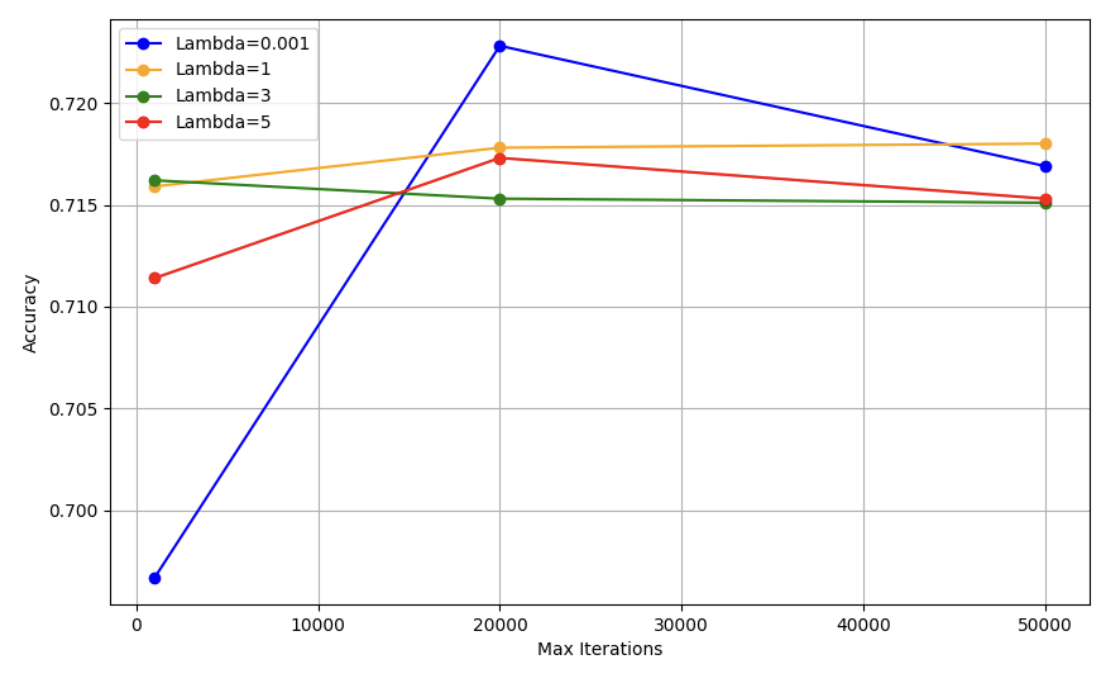
\includegraphics[width=0.6\textwidth]{images/accSVM.png}
    \caption{Accuracy for different parameters combinations}
    \label{fig:accSVM}
\end{figure}

A brief discussion about \(\lambda\) parameter is necessary. 
\begin{itemize}
    \item A \(\lambda\) that is too high means that the weight penalty is very strong. This leads the model to try to minimize the weights as much as possible, reducing the complexity of the model. The risk of this is that it fails to adequately capture the relationships between the variables and the targets, resulting in underfitting.
    \item A \(\lambda\) that is too low, on the other hand, means that the regularization is very weak. This can lead the model to focus too much on the training data, increasing the complexity of the model. As a result, the model may become too “fitted” to the training data, also capturing the noise present in the data. This phenomenon is known as overfitting.
\end{itemize}

\subsubsection{Results Analysis}

The grid search results showed that the best parameters were \(\lambda = 0.001\) and \(\texttt{max\_iter} = 20000\), with an average accuracy of 0.7154 on the training set. 
A very low lambda value, as shown by the blue line, allows the model to fit the training data very well, with a significant improvement in accuracy as the number of iterations increases. However, we notice that after a certain number of iterations (around 20,000), the accuracy starts to decrease. This is a sign of overfitting, where the model starts to “learn too much” from the training data, capturing noise rather than generalizing to unseen data.
With higher lambda values (yellow, green, and red lines), the model introduces stronger regularization, which prevents overfitting. However, these lambda values can lead to slight underfitting, especially when combined with a low number of iterations, as the model may not be able to capture all the complexities of the data.

After choosing the best model based on the cross-validation results, the final training and evaluation was performed on the test set, obtaining the following results:
\begin{itemize}
    \item Accuracy on the test set: 0.7205
    \item Misclassification rate on the test set: 0.2795
\end{itemize}

\newpage
\subsection{Regularized Logistic Regression}

Logistic regression is a classification method used to estimate the probability that a given instance belongs to one of two classes in a binary classification problem. In mathematical terms, the predictor is assumed to be a linear model \(\mathbf{w}^\top \mathbf{x}\), which is then transformed into a probability using the sigmoid function:

\[
\text{sigmoid}(z) = \frac{1}{1 + e^{-z}}
\]

where \(z = \mathbf{w}^\top \mathbf{x}\). The sigmoid function maps linear values to a range between 0 and 1, allowing the output to be interpreted as a probability.

In regularized logistic regression, a penalty term is introduced to avoid overfitting and improve the generalization of the model. The objective function to be minimized then becomes the sum of the logistic loss on the data and the L2 regularization term:

\[
\min_{\mathbf{w}} \left( \frac{1}{m} \sum_{i=1}^m \log(1 + e^{-y_i \mathbf{w}^\top \mathbf{x}_i}) + \frac{\lambda}{2} \|\mathbf{w}\|^2 \right)
\]

The Pegasos algorithm, originally developed for the optimization of SVMs, can be adapted to logistic regression by modifying the loss function to be minimized, replacing the hinge loss with the logistic loss. The algorithm performs an iterative update of the weights \(\mathbf{w}\) based on random samples, according to the rule:

\[
\mathbf{w}_{t+1} = (1 - \eta_t \lambda) \mathbf{w}_t + \eta_t y_t \mathbf{x}_t \left( 1 - \text{sigmoid}(y_t \mathbf{w}_t^\top \mathbf{x}_t) \right)
\]

where \(\eta_t\) is the learning rate, calculated as the inverse of the product between the regularization parameter \(\lambda\) and the number of iterations \(t\). During training, the cumulative weight vector, \(\mathbf{cumulative\_w}\), is kept track of, which represents the sum of the weights computed during all iterations. At the end of training, the final weight vector is given by the average of the obtained weights.

\subsubsection{Implementation of the Algorithm}

When implementing the sigmoid function, it was necessary to introduce a limit on the values of \(z\) (the scalar product of the weights and the feature vector). This is because the exponential function \(\exp(z)\) can easily overflow numerically when \(z\) takes on very negative or very positive values. To avoid this problem, the values of \(z\) have been limited to the interval \([-700, 700]\) using the \texttt{np.clip()} function. This is essential to ensure that the sigmoid calculation does not cause overflow errors, which can compromise the reliability of the algorithm's results.

It was observed that, although the average accuracy obtained during cross-validation remained unchanged, the absence of the bound caused a 10\% increase in the misclassification rate on the test set. 

The decrease in accuracy on the test set can be attributed to the model losing sensitivity to extreme values of \(z\) , which were important for correctly distinguishing classes on the unseen data. By limiting the values of \(z\) , the model may have lost some of its ability to discriminate between classes, leading to an increased rate of misclassification on the test data.

\subsubsection{Hyperparameter tuning}

Similarly to what was done in SVM, a grid search combined with 5-fold cross-validation was implemented and tested. Parameters are the same as before and reported in the following table:
\begin{table}[H]
\centering
\begin{tabular}{|c|c|}
\hline
\textbf{Lambda Param} & \textbf{Max Iter} \\ \hline
0.001 & 1000 \\ \hline
1 & 20000 \\ \hline
5 & 50000 \\ \hline
\end{tabular}
\caption{Combinations of Parameters}
\label{tab:param_combinations}
\end{table}

The process ended with the computation of an average accuracy for each combination:

\begin{figure}[H]
    \centering
    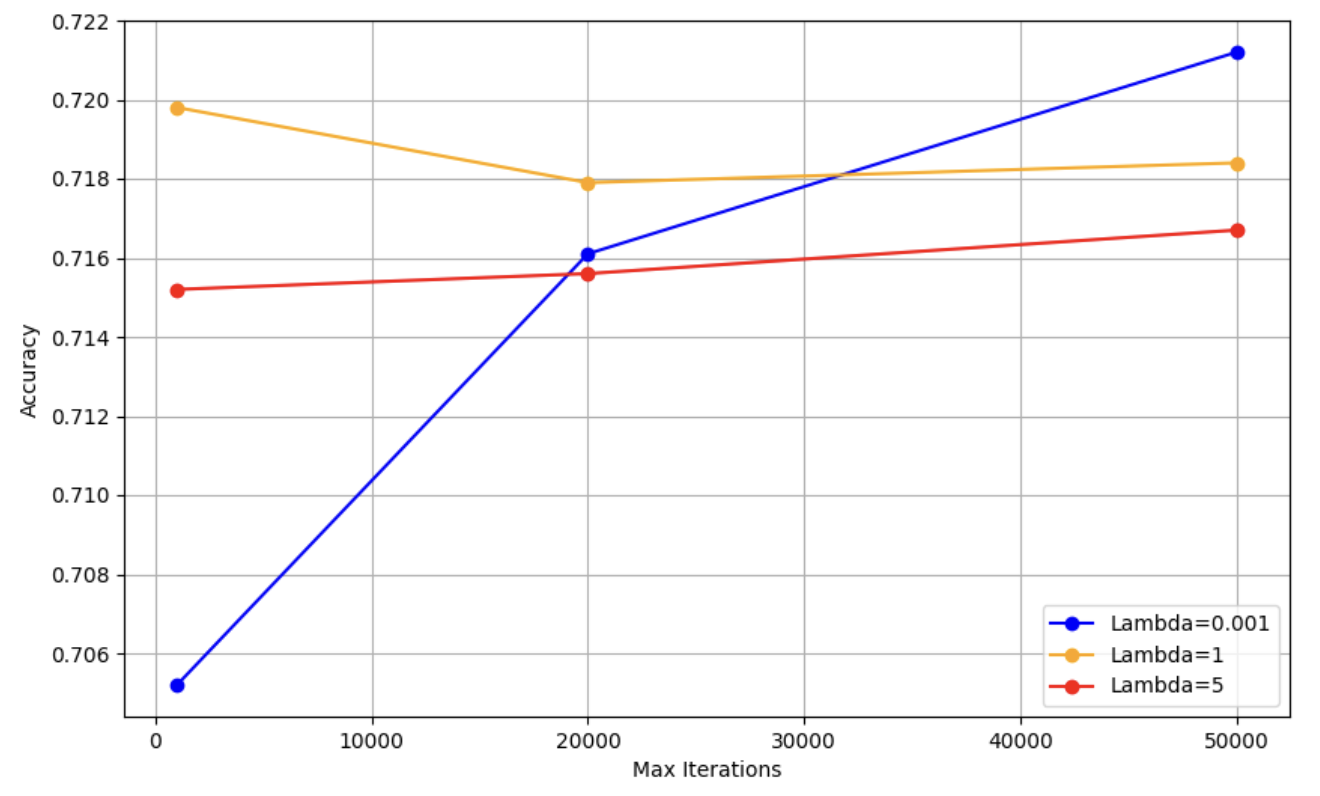
\includegraphics[width=0.6\textwidth]{images/accLOG.png}
    \caption{Accuracy for different parameters combinations}
    \label{fig:accLOG}
\end{figure}

\subsubsection{Results analysis}
As highlighted by the results, the best combination of parameters for this model is \(\lambda = 0.001\) and \texttt{max\_iter} = 50000, which resulted in an average accuracy of 0.7262 during cross-validation. After training the model using these optimal parameters, the following results were obtained:
\begin{itemize}
    \item Accuracy on test set: 0.7199
    \item Misclassification rate on test set: 0.2801
\end{itemize}

The plot highlights how the model accuracy varies with different lambda values and maximum iterations. For a lambda value of 0.001, a steady improvement in accuracy is observed with increasing iterations, suggesting that the model is fitting the training data well. However, this can lead to a risk of overfitting, where the model becomes too complex and specific to the training data.

In contrast, for higher lambda values, such as 1 and 5, the accuracy remains more stable and does not improve significantly with increasing iterations. This indicates greater resistance to overfitting, but at the same time a potential risk of underfitting, where the model may not fully capture the complexity of the data.

\vspace{0.5cm}

In summary, this result highlights an important trade-off between numerical stability and predictive ability of the model. While the implemented solution ensured numerically stable training, it also limited the model's ability to effectively generalize to test data.

\newpage
\section{Polynomial Feature Expansion and Model Improvement}
Polynomial feature expansion is a technique that improves the performance of machine learning models, especially linear ones, by transforming the original features into new nonlinear features. This approach is particularly useful when the basic linear model is not complex enough to capture the underlying relationships in the data.

\vspace{0.5cm}
Mathematically, feature expansion can be viewed as a function \(\phi: \mathbb{R}^d \rightarrow H\), where \(H\) is a higher-dimensional space. For example, for a quadratic expansion, the function \(\phi(x)\) transforms an input vector \(x\) into a new vector containing all the squared combinations of its components. This allows the model to learn more complex features that are representable in the new feature space.

\vspace{0.5cm}
In a machine learning context, polynomial expansion is used to reduce the bias of the model, that is, the approximation error due to its inability to capture the true relationship between the independent variables and the dependent variable. However, this technique can also increase the risk of overfitting, as increasing the number of parameters makes the model more susceptible to noisy data.

\vspace{0.5cm}
In the specific case of this project, degree 2 feature expansion was used to transform the original features into new quadratic combinations, allowing linear models to learn more complex nonlinear relationships. Subsequently, the linear weights corresponding to these new features were included and compared after the training phase to evaluate the improvement in model performance.

\begin{verbatim}
Shape of original features: (7786, 8)
Shape of features after polynomial expansion: (7786, 44)
New list of features: ['x1', 'x2', 'x3', 'x4', 'x5', 'x6', 'x7', 'x8',
'x1*x1', 'x1*x2', 'x1*x3', 'x1*x4', 'x1*x5', 'x1*x6', 'x1*x7', 'x1*x8',
'x2*x2', 'x2*x3', 'x2*x4', 'x2*x5', 'x2*x6', 'x2*x7', 'x2*x8', 'x3*x3',
'x3*x4', 'x3*x5', 'x3*x6', 'x3*x7', 'x3*x8', 'x4*x4', 'x4*x5', 'x4*x6',
'x4*x7', 'x4*x8', 'x5*x5', 'x5*x6', 'x5*x7', 'x5*x8', 'x6*x6', 'x6*x7',
'x6*x8', 'x7*x7', 'x7*x8', 'x8*x8']
\end{verbatim}

\newpage
\subsection{Retrain of the models with polynomial features}
After performing the second-degree polynomial expansion, the models were retrained using the new training and test sets containing the expanded features. To ensure accurate performance evaluation, a cross-validation function was developed that not only identifies the best parameters and calculates the best accuracy, but also evaluates whether the inclusion of the polynomial expansion improves the overall performance of the model compared to using the original features alone.

\vspace{0.5cm}
After performing the 5-fold cross validation, the average accuracy obtained for each combination of parameters is reported in the following graphs:

\begin{figure}[H]
    \centering
    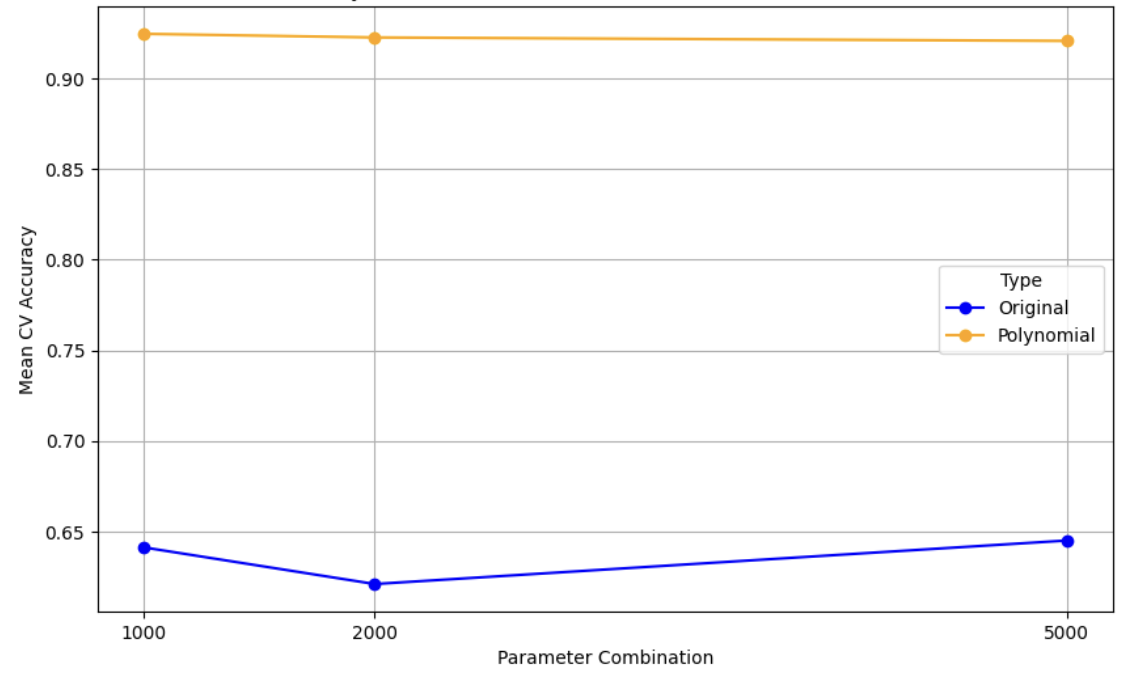
\includegraphics[width=0.6\textwidth]{images/polyPER.png}
    \caption{Accuracy for different parameters combinations - PERCEPTRON}
    \label{fig:polyPER}
\end{figure}

\begin{itemize}
    \item Best hyperparameters: max\_epochs (1000)
\end{itemize}

For the Perceptron model, the accuracy with the original features was around 62-63\%, regardless of the number of epochs (1000, 2000, or 5000). However, after applying the polynomial expansion, the accuracy increased dramatically to over 91\% for all epoch configurations. This suggests that the Perceptron model benefits significantly from the additional features generated by the quadratic expansion, which likely capture more complex patterns in the data that were not accessible with the original linear features alone.

\begin{figure}[H]
    \centering
    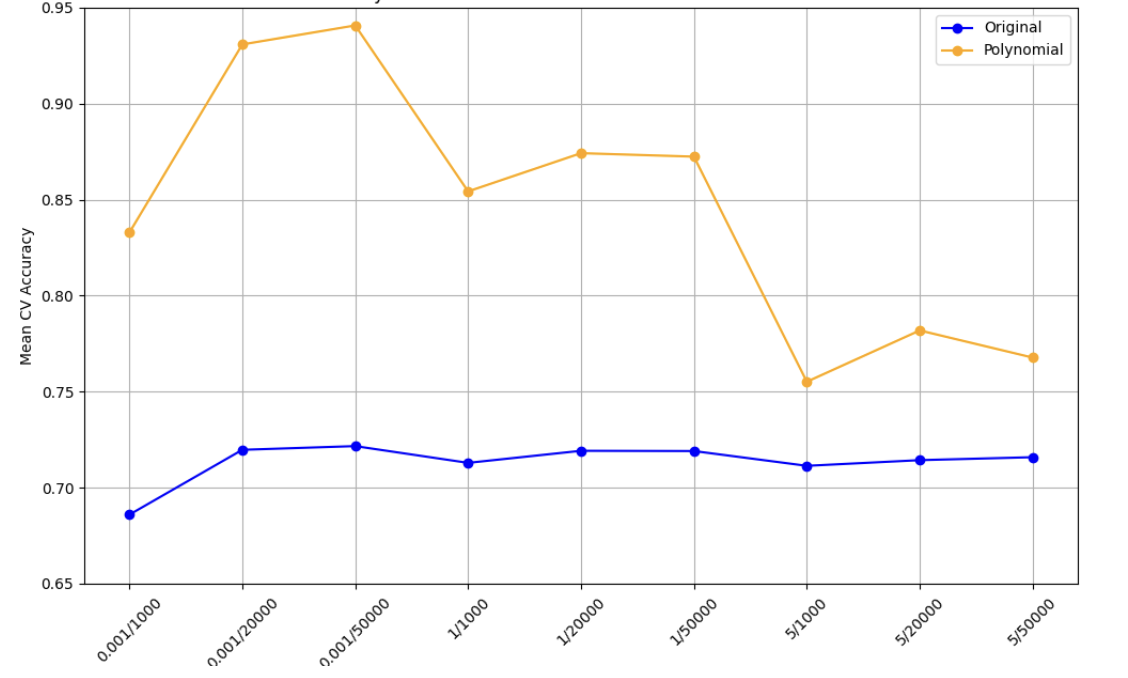
\includegraphics[width=0.6\textwidth]{images/polySVM.png}
    \caption{Accuracy for different parameters combinations - SVM}
    \label{fig:polySVM}
\end{figure}

\begin{itemize}
    \item Best hyperparameters: lambda (0.001), max\_iter(50000)
\end{itemize}

It is evident that increasing the lambda parameter leads to a tendency for the model to underfit. In particular, for high values f lambda (e.g., lambda = 1 and lambda = 5), the accuracy is significantly lower than that obtained with lower lambda (lambda = 0.001), even by increasing the number of iterations.

This behavior indicates that, with higher lambda values, the strong penalty imposed on the weights excessively reduces the flexibility of the model, preventing it from adequately fitting the training data. As a result, the model fails to capture the complex relationships present in the data, leading to a lower accuracy than models with lower lambda, which maintain a greater capacity to adapt.

\begin{figure}[H]
    \centering
    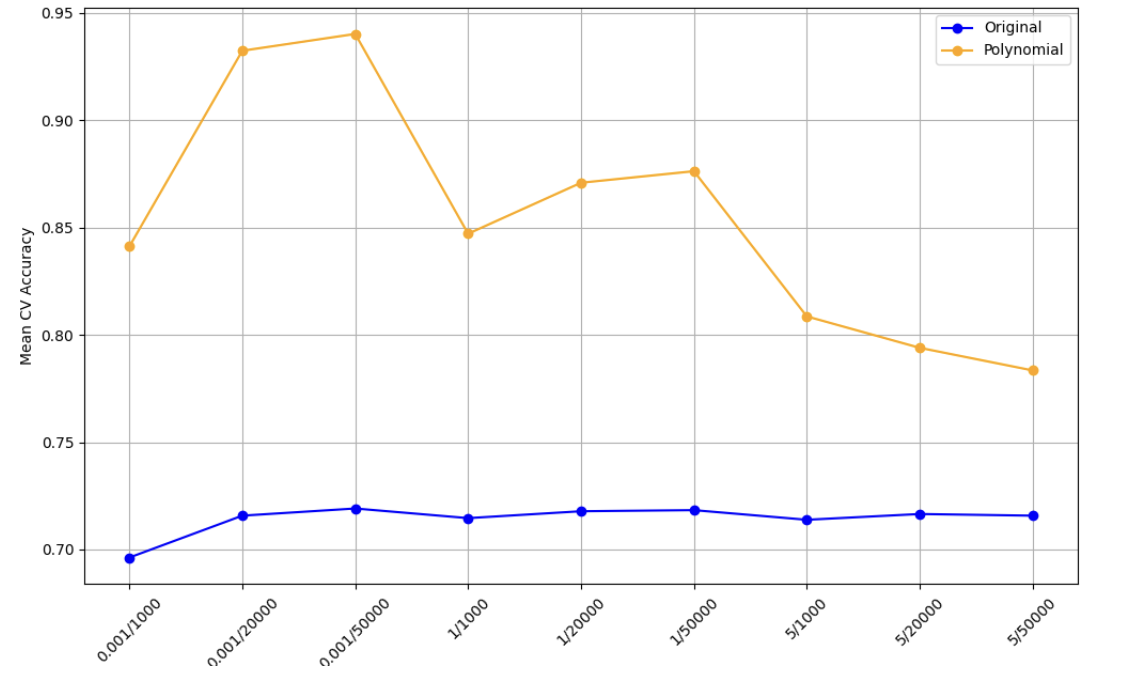
\includegraphics[width=0.6\textwidth]{images/polyLOG.png}
    \caption{Accuracy for different parameters combinations - LOGISTIC CLASSIFICATION}
    \label{fig:polyLOG}
\end{figure}

\begin{itemize}
    \item Best hyperparameters: lambda (0.001), max\_iter(50000)
\end{itemize}

The analysis for Logistic Classification highlights a very similar pattern to the one observed for the SVM with Pegasos updates, as illustrated in the graph. This shows a significant increase in accuracy when using polynomial features compared to the original ones.
However, it is evident that increasing lambda, the accuracy with polynomial features starts to decrease, potentially indicating the beginning of underfitting. As in the case of the SVM, a model that is too simple may underfit the training data.

Overall, the three models perform way better when they use polynomial features. Below, the results of misclassification rates on test set are reported:
\begin{figure}[H]
    \centering
    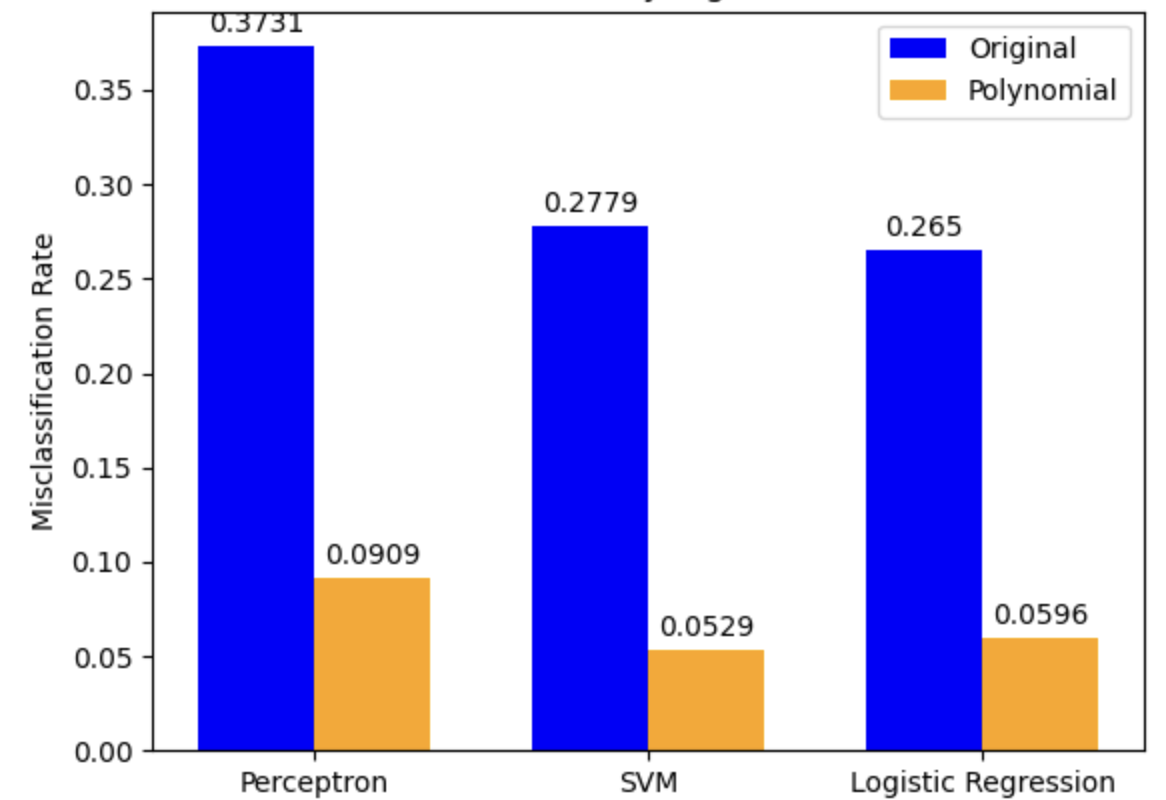
\includegraphics[width=0.6\textwidth]{images/missPOLY.png}
    \caption{Misclassification rates - Original vs Polynomial}
    \label{fig:missPOLY}
\end{figure}

\begin{figure}[H]
    \centering
    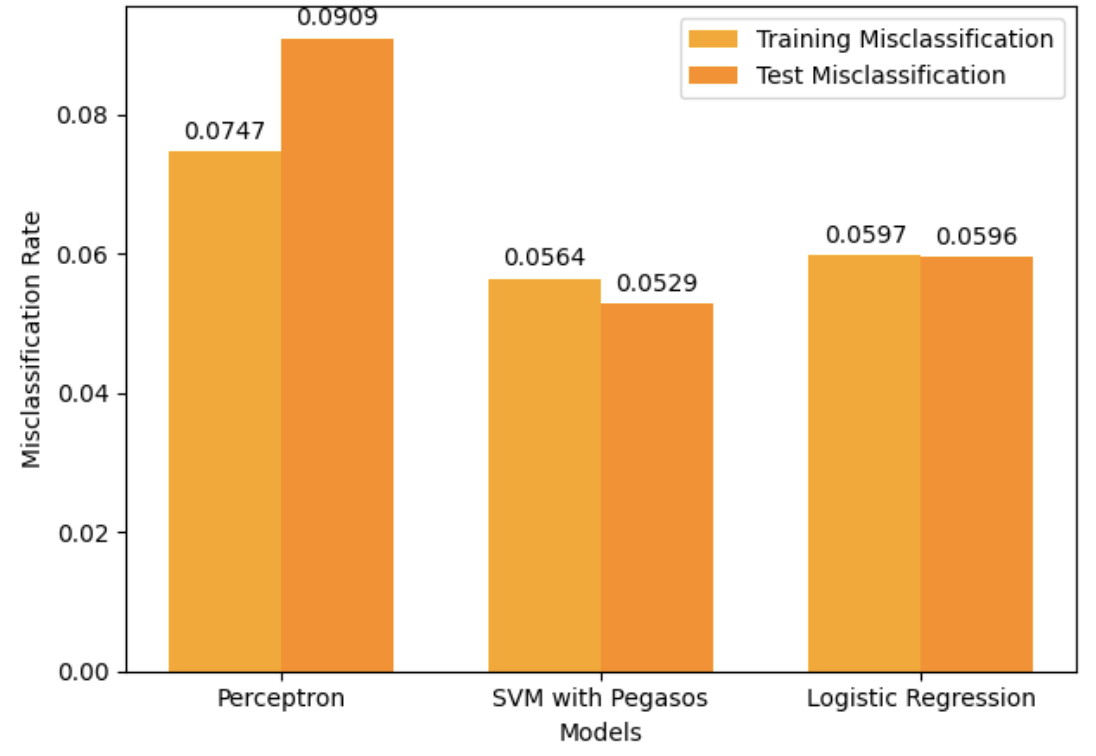
\includegraphics[width=0.6\textwidth]{images/polyTEST.png}
    \caption{Misclassification rates - Training vs Test}
    \label{fig:polyTEST}
\end{figure}

We can state that none of the models show a large gap bewtween training and test misclassification rates, which suggests that none of the models suffer from severe overfitting. 
SVM model appears to generalize slightly better than the others as indicated by the lowest test error compared to the training error. 

\newpage
\subsection{Comparison of linear weights}

In this section, we analyze the weights obtained by the three models (Perceptron, SVM, and Logistic Regression) before and after the polynomial expansion of the features. The goal is to understand how the polynomial expansion influenced the importance of the variables and improved the ability of the models to capture complex relationships between the features.

\subsubsection{Perceptron}

\textbf{Original Weights}: 

In the original Perceptron, the features \( x3 \), \( x1 \) and \( x4 \) showed a predominant influence on the model, with higher weight values in absolute terms than the other features. This indicates that the model considers these variables to be the most relevant for classification.

\vspace{0.5cm}
\noindent \textbf{Weights After Polynomial Expansion}: 

After polynomial expansion, feature combinations such as \( x2 \times x8 \), \( x1 \times x7 \) and \( x4 \times x7 \) became significantly more important, suggesting that the interactions between these features are crucial for the model. Although some individual feature weights, such as \( x1 \) and \( x4 \), remain relevant, the importance of the interactions between the features becomes dominant. This indicates that the Perceptron has benefited significantly from the polynomial expansion, as it is now able to capture more complex relationships between the variables.

\subsubsection{Support Vector Machine (SVM)}

\textbf{Original Weights}: 

In the original SVM, the features \( x7 \) and \( x6 \) showed the greatest influence on the model. The weight distribution was relatively balanced among the features, suggesting that all the variables have significant importance in the classification.

\vspace{0.5cm}
\noindent \textbf{Weights After Polynomial Expansion}: 

After the polynomial expansion, interactions between features such as \( x2 \times x8 \) and \( x4 \times x7 \) became particularly prominent. The polynomial expansion significantly increased the weights of these combinations, indicating that the SVM is now able to capture nonlinear relationships between the variables, which were less evident before. This suggests that the polynomial expansion made the SVM model more complex and, consequently, more accurate in distinguishing between classes.

\subsubsection{Regularised Logistic Classification}


\textbf{Original Weights}: 

In the original logistic regression, the features \( x7 \), \( x4 \), and \( x5 \) emerged as the most influential on the model. Similar to the SVM, the logistic regression showed a fairly balanced distribution of weights, although some weights were slightly higher.

\vspace{0.5cm}

\noindent \textbf{Weights After Polynomial Expansion}: 

After the polynomial expansion, feature combinations such as \( x2 \times x8 \) and \( x7 \times x4 \) became the most relevant. As in the other models, the polynomial expansion led to an increase in the importance of feature interactions, demonstrating that logistic regression is able to exploit these interactions to improve its performance. Although the weights of individual features remain relevant, the complexity of the model increases with the inclusion of feature combinations.


\newpage



\section{Kernel Methods}
Kernel methods are a class of algorithms that enable linear models to learn non-linear relationships by implicitly mapping data into higher-dimensional spaces. The key idea behind kernel methods is the “kernel trick,” which allows the computation of inner products in a high-dimensional feature space without explicitly mapping the data into that space, but using Kernel functions.

Two common Kernel functions are: 
\begin{itemize}
    \item Polynomial Kernel of degree \(n\):
    \[ K(x, x') = (1 + x^\top x')^n\]
    \item Gaussian Kernel: 
    \[K(x, x') = \exp\left(-\frac{\|x - x'\|^2}{2\gamma}\right)\]
\end{itemize}

In this project, Kernel SVM and Kernel Perceptron are implemented. These algorithms are extensions of their linear versions that use kernel functions to map the data into a high-dimensional space, where classes can be more easily separated with a hyperplane. This approach allows models to capture nonlinear relationships in the data.
Both models are implemented with gaussian and polynomial kernel functions.
As with previous implementations, even after upgrading the algorithms to their kernel version, a rigorous parameter selection was required. Hyperparameter tuning was performed using a grid search on a set of different parameter values, combined with a 5-fold cross-validation. The obtained results are presented below.

\subsection{Kernelized Perceptron}
The Kernelized Perceptron is better suited for datasets where the decision boundary is non-linear. It is more flexible and can model more complex relationships between features.
By the way, it is computationally more expensive and requires careful selection and tuning of the kernel and its parameters (e.g., gamma for the Gaussian kernel or degree for the Polynomial kernel). For very large datasets, this might be impractical.


\subsubsection{Gaussian}

The implementation of Gaussian Kernelized Perceptron went through the same procedure of grid search with 5-fold CV. The parameters that can be used are the maximum number of iterations and gamma. By the way, only the second parameter has been tuned- because of computational cost of running Perceptron. Also, parallel experiments showed that the Perceptron converged always after 5 or 6 epochs, so tuning max\_iter would have been useless and redundant.


The performances of the model with different gammas is reported in the following table:
\begin{table}[H]
\centering
\begin{tabular}{|c|c|}
\hline
\textbf{Gamma Param} & \textbf{Mean CV Accuracy} \\ \hline
0.0001 & 0.8228\\ \hline
1 & 0.8228 \\ \hline
5 & 0.8228 \\ \hline
\end{tabular}
\caption{Hyperparameter tuning - Kernelised Perceptron}
\label{tab:CVaccuracyKPG}
\end{table}

During the analysis, it was found that the average cross-validation accuracy remains constant (82.28\%) for a wide range of gamma values. This behavior indicates an intrinsic robustness of the Gaussian kernelized model, suggesting that the choice of gamma does not significantly affect the model performance. This stability can be attributed to the data structure and the effectiveness of the normalization process, which reduces the sensitivity of the model to gamma changes. Therefore, the model demonstrates high generalizability without requiring fine tuning of this hyperparameter, making it suitable for a variety of application contexts.

Final performance on test set:
\begin{itemize}
    \item Accuracy on test set: 0.8207
    \item Misclassification rate on test set: 0.1793
\end{itemize}

\subsubsection{Polynomial}

Similar to the behavior observed with the Gaussian kernel, the application of the polynomial kernel in the perceptron also showed a constant average accuracy (94.60\%) across different degrees of the polynomial. This suggests that the model effectively captures the relationships present in the data already with a relatively low polynomial degree, and further increases in the kernel complexity do not lead to significant improvements. This behavior indicates not only the robustness of the model against overfitting, but also that higher degree polynomial transformations do not add enough information value to justify increased computational complexity.

It's important to note that there isn't a direct implementation of this algorithm in the notebook because the machine used to run the code wasn't powerful enough and it was run on another machine. The model was run with hyperparameters degree (2) and max\_epochs (10).

Final performance on test set:
\begin{itemize}
    \item Accuracy on test set: 0.94
    \item Misclassification rate on test set: 0.06
\end{itemize}




\subsection{Kernelized Pegasos SVM}

\subsubsection{Guassian}

As reported by the cross-validation results (see graph below), the combination of parameters that led to the best accuracy was \(\lambda = 0.01\) and \(\gamma = 0.001\), with an average accuracy of 81\% on the cross-validation sets.

\begin{figure}[H]
    \centering
    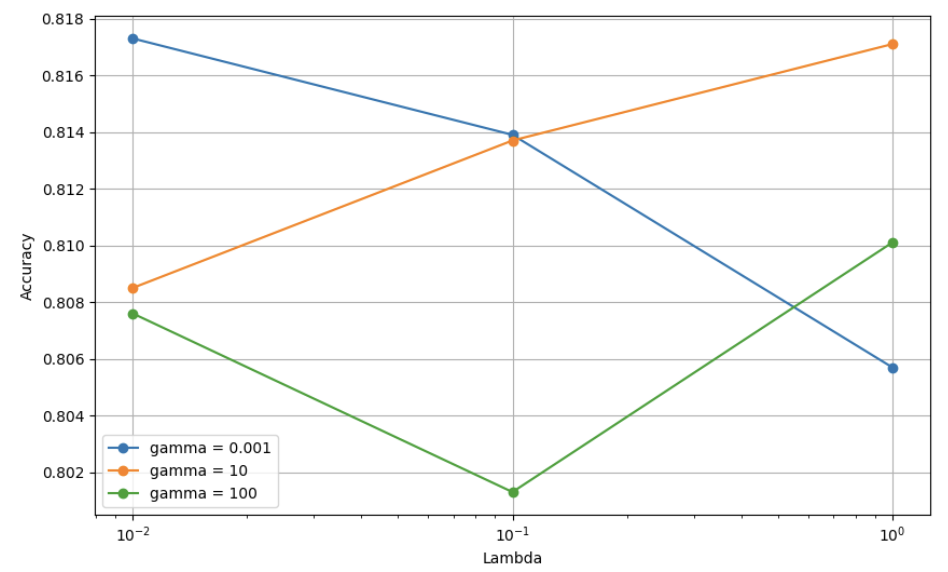
\includegraphics[width=0.6\textwidth]{images/accKSVMG.png}
    \caption{Accuracy (grid search, 5-fold CV) of Kernelised Gaussian SVM}
    \label{fig:accKSVMG}
\end{figure}

The gamma parameter modulates the width of the Gaussian kernel, affecting how sensitive the model is to distances between points. A low gamma (0.001) implies greater generalization, since the kernel has a larger width, resulting in accuracy that increases with increasing lambda. This suggests that increasing regularization (higher lambda) can help prevent overfitting when gamma is low.
Conversely, with higher gamma values (10 and 100), where the model becomes more sensitive to precise distances between points, increasing lambda leads to overregularization, evidenced by a decrease in accuracy. This effect is particularly evident with gamma at 10, where accuracy decreases as lambda increases. However, with gamma = 100, accuracy initially worsens and then improves, indicating a possible balance point between overfitting and underfitting.

Evaluating this model on test set, we get the following scores:
\begin{itemize}
    \item Accuracy on test set: 0.8279
    \item Misclassification rate on test set: 0.1721
\end{itemize}

\subsubsection{Polynomial}

\begin{figure}[H]
    \centering
    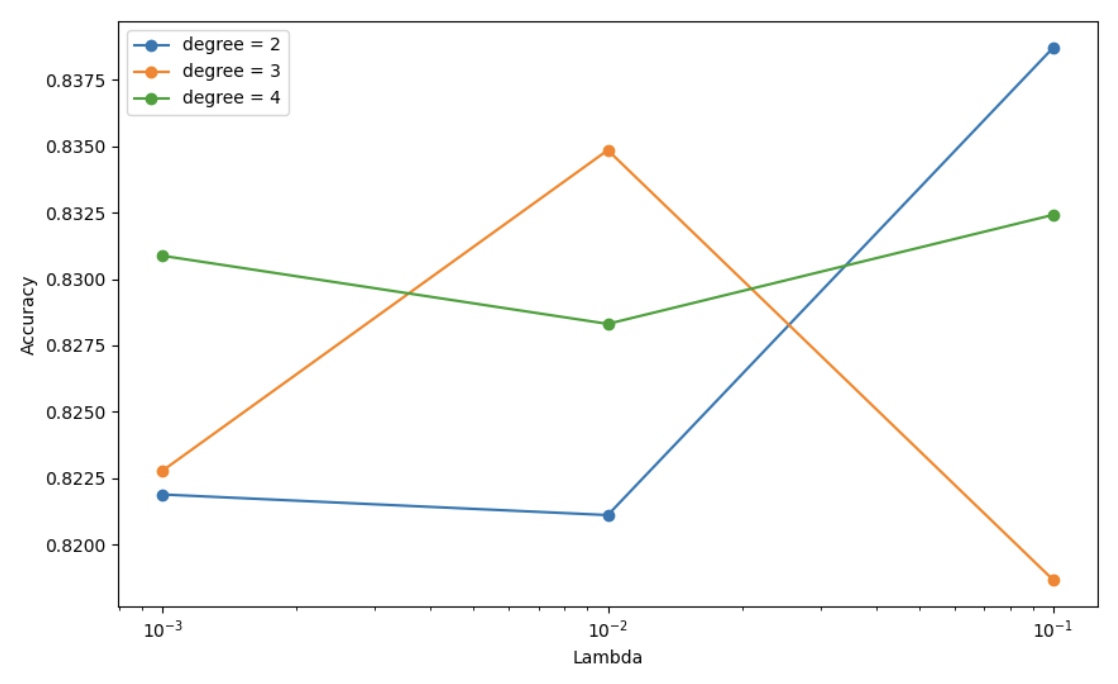
\includegraphics[width=0.6\textwidth]{images/accKSVMP.png}
    \caption{Accuracy (grid search, 5-fold CV) of Kernelised Polynomial SVM}
    \label{fig:accKSVMP}
\end{figure}

From the graph, we can see that degree 4 is the most stable in terms of accuracy, but the best performing is 2nd degree with \(\lambda = 0.1\). The choice of this as the best parameter makes the Kernelised Polynomial SVM very similar to the classic SVM with polynomial expansion of the second degree features, but with some key differences:


\begin{enumerate}
\item \textbf{Computational Efficiency}: The SVM with explicit polynomial expansion of the features increases the number of dimensions and can make the training computationally expensive. The Kernelised Polynomial SVM, instead, computes the scalar products between the expanded features implicitly, resulting in a generally more efficient result.
\item \textbf{Feature Explicitness}: In the SVM with polynomial expansion, the features are transformed explicitly, while in the Kernelised Polynomial SVM the kernel computes the effects of the polynomial features without directly constructing them.
\item \textbf{Generalization Ability}: Explicit feature expansion in classical SVM can lead to a higher risk of overfitting, while Kernelised Polynomial SVM, thanks to the regularizing properties of the kernel, can improve the generalization ability of the model on new data.
\end{enumerate}


\noindent Below the scores of best parameters:
\begin{itemize}
    \item Accuracy on test set: 0.8294
    \item Misclassification rate on test set: 0.1706
\end{itemize}


\newpage
\section{Conclusions}

\begin{figure}[H]
    \centering
    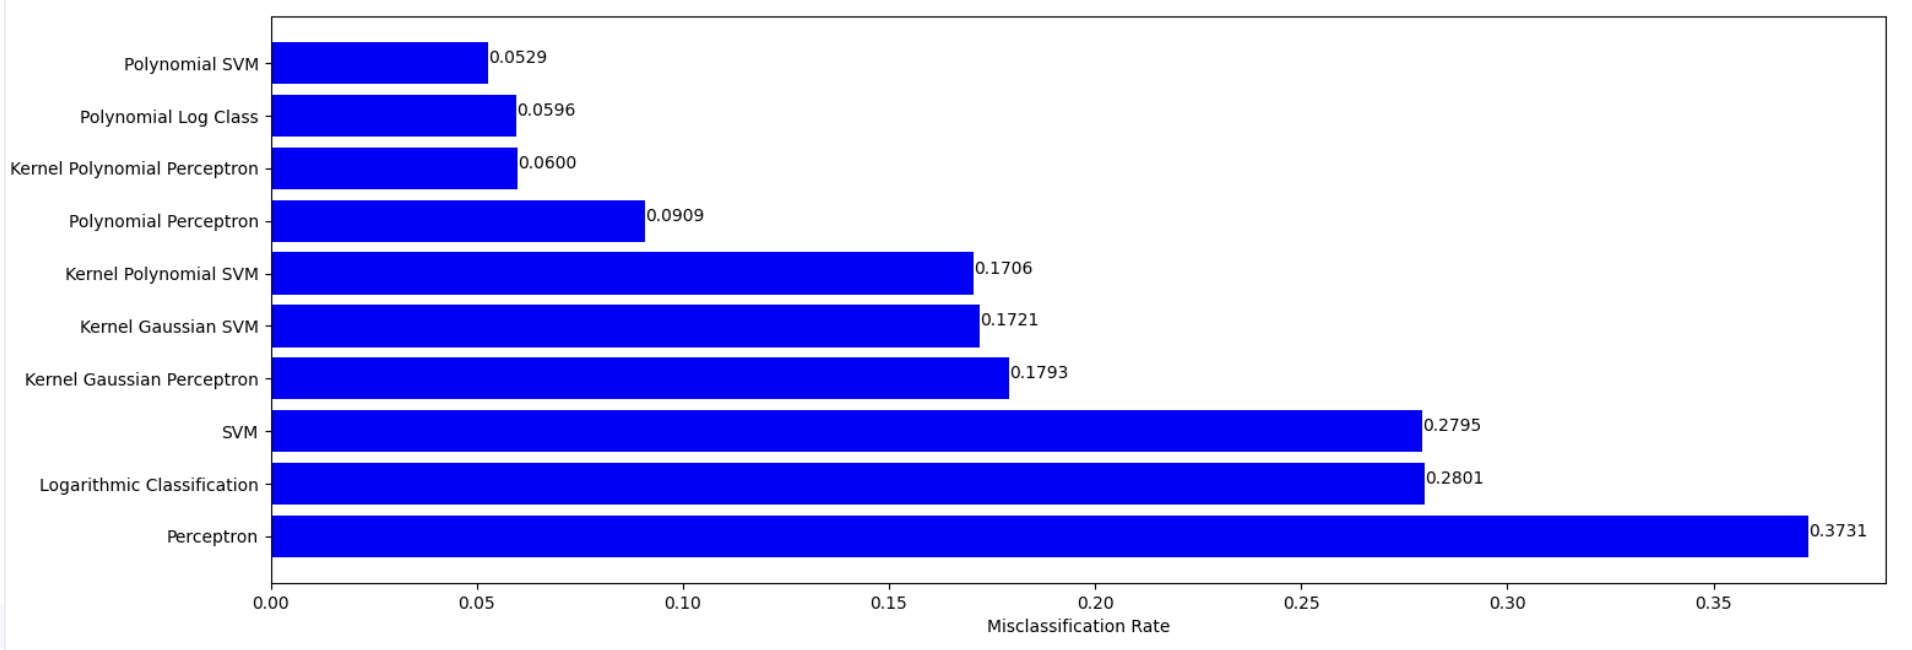
\includegraphics[width=1\textwidth]{images/general.png}
    \caption{Models ranking (0-1 Loss).}
    \label{fig:general}
\end{figure}

The figure \ref{fig:general} illustrates a ranking of the architectures explored in this study based on their performance using the zero-one loss function. The most effective solution to the problem is provided by Polynomial SVM (0.053\%), trained with a degree of 2. 
Polynomial versions of the three main algorithms implemented deliver a solid solution, with a loss approximately equal to 5-10\%, striking a good balance between complexity and performance.
This means that once the features have been transformed by a certain polynomial degree (degree 2), further increases in degree do not add significant information value, and thus the accuracy remains unchanged. This could indicate that the nonlinear relationships present in the data are already captured with a low degree of transformation, and therefore increasing the degree does not further improve the model.

For this reasons, the final choice falls between Polynomial SVM and Polynomial Logistic Classification, which are the best performing when balancing error rate and computational costs.

From the results and insights gained through this research, the following conclusions can be drawn:
\begin{itemize}
    \item Starting with simpler models and gradually increasing their complexity can be an effective strategy to identify the most suitable algorithm for the task at hand.
    \item Higher model complexity does not always equate to better performance; it is crucial to match the complexity of the algorithm to the specific problem to avoid issues related to overfitting or underfitting.
    \item It's likely that dataset isn't linearly separable because classical and polynomial implementations of Perceptron never converged. The convergence of the kernelised Gaussian perceptron only shows that the data is separable in a high-dimensional space created by the kernel, but does not provide information about the linear separability in the original space.
\end{itemize}


\end{document}